\documentclass{beamer}

\usepackage{upquote}
\usepackage{color}
\usepackage{alltt}
\usepackage{graphicx}
\usepackage{listings}
\lstset{ %
  basicstyle=\tiny\ttfamily\color{blue}, %
  frame=single, %
  includerangemarker = false, %
  title = \footnotesize\ttfamily\color{blue}\emph{Interactive Stata Example}, %
  captionpos = t, %
  rangeprefix=*@*%, %
  %belowcaptionskip = -0.08in, %
  %label={bla}
}

\usetheme{Boadilla}

%\usecolortheme{orchid}
%\usecolortheme{beaver}
%\setbeamercolor{item projected}{fg=black,bg=white}
\usecolortheme{beaver}
\setbeamertemplate{itemize subitem}[triangle]
\setbeamercolor{item projected}{fg=darkred, bg=lightgray}
\setbeamercolor{subitem projected}{fg=darkred}
\setbeamercolor{local structure}{fg=darkred}


\usefonttheme{professionalfonts}

%\usepackage{verbatim}
%{\catcode`\`=13 \g@addto@macro\@verbatim{\chardef`=18 }}

\title{MPP-C6: Statistics II}
\subtitle{Programming with Stata}
\author{Max Callaghan}
\institute[HSoG]{Hertie School of Governance}
\titlegraphic{
\includegraphics[width=2cm]{HSOG_logo.png}}
\date{?? February 2015}


\begin{document}

\frame{\titlepage}

\begin{frame}
  \frametitle{Outline}
  \begin{itemize}
    \item Why Program?
    \item Reproducible Research
    \item Programming in Stata to accomplish difficult tasks and simplify repetitive tasks
  \end{itemize}
\end{frame}

\begin{frame}
  \frametitle{Why Program?}
  \begin{itemize}
    \item Computers can perform calculations faster and more accurately than humans
    \item When a task is difficult or repetitive, if often makes sense to instruct the computer to do it
    \item When those instructions are written down, we and others can see exactly what has been done
    \begin{itemize}
      \item It's easier to repeat the work
      \item It's easier to spot errors
      \item It's easier to repeat the work, changing just one detail, without doing every subsequent step again.
    \end{itemize}
  \end{itemize}
\end{frame}

\begin{frame}
  \frametitle{Reproducible Research}
  \begin{itemize}
    \item ``The standard of reproducibility calls for the data and the computer code used to analyse the data to be made available to others" \cite{Peng}
    \item Literate programming ties together data, code and the actual research output, enhancing reproducibility
  \end{itemize}
\end{frame}

\begin{frame}
  \frametitle{Reproducible Research}
  \frametitle{Reproducible Research with Stata}
  \begin{itemize}
    \item What do we already do that helps to keep our research reproducible?
    \item How do we ensure that what's in our research output reflects the calculations we report making?
  \end{itemize}
\end{frame}

\begin{frame}
  \frametitle{Reproducible Research}
  \frametitle{Reproducible Research with Stata}
  \begin{itemize}
    \item The ideal for perfect reproducibility would be to have a single document that contains instructions for performing calculations as well as for producing the research output we present.
    \item This is not possible in Stata without \LaTeX\ but we can at least make the way we include Stata output in Word documents more systematic
  \end{itemize}
\end{frame}

\begin{frame}
  \frametitle{Reproducible Research}
  \frametitle{Reproducible Research with Stata}
  [Include instructions to do this, with a simple example of output that changes to reflect a change in a do file]
\end{frame}

\begin{frame}
  \frametitle{Programming with Stata}
  %\framesubtitle{Stata Refresher}
  \framesubtitle{Outline}
  \begin{itemize}
    \item Stata basics
    \item Directory structure
    \item Reading data
    \item Transforming and processing data
    \item Presenting results with Stata
  \end{itemize}
\end{frame}

\begin{frame}
  \frametitle{Programming with Stata}
  \frametitle{Stata Basics}
  %\framesubtitle{Outline}
  \begin{itemize}
    \item Pointing and clicking is fine for exploring data
    \item The command line is fine for trying out commands
    \item Anything you want to be able to reproduce, you should put in the do file
  \end{itemize}
\end{frame}

\begin{frame}[fragile]
  \frametitle{Programming with Stata}
  \frametitle{Stata Basics}
  \framesubtitle{Writing a good do file}
  A good do file should be readable by humans as well as computers.
  \begin{itemize}
    \item Use comments to explain what each line is doing
    \item Empty lines are free, space makes your code easier to read
    \item Use meaningful names when you create them, and write them consistently (variable\_name, variableName or VariableName)
    \item Follow indentation conventions e.g.
    \begin{verbatim}
forvalues i in 1/5 {
  display `i'
}
    \end{verbatim}
  \end{itemize}
\end{frame}

\begin{frame}[fragile]
  \frametitle{Programming with Stata}
  \frametitle{Stata Basics}
  \framesubtitle{Understanding Stata Commands}
  Stata commands are preprogrammed functions that take information we give to them, do something with the information, then output something. We pass information to commands with \textit{arguments} and \textit{options}.
  
  If you are not sure how to use a command you can get help by typing "help" and then the name of the command. For example,
  \begin{verbatim} help regress \end{verbatim}
  will take you to the regress command's \href{http://www.stata.com/manuals13/rregress.pdf}{manual}
\end{frame}

\begin{frame}
  \frametitle{Programming with Stata}
  \frametitle{Stata Basics}
  \framesubtitle{Reading the Stata manual}
  The Syntax \texttt{\underline{reg}ress} \textit{\textcolor{blue}{depvar [indepvars] [if] [in] [weight]} [,options]} describes the basic use of the command
  \begin{itemize}
    \item Pay attention to the order of the arguments. This is how Stata knows which arguments are which
    \item Items in square brackets are optional
    \item Options come after a comma. Possible options are described in the help file
    \item You don't always need to set a lot of options, but you should pay atention to what the defaults are
  \end{itemize}
  If you don't know the command you want to use, you will have try and describe your problem to google.
\end{frame}

\begin{frame}
  \frametitle{Directory Structure}
  %\framesubtitle{Directory Structure}
  File paths tell the computer where to read and write information. They differ between Windows and Mac/Linux. (\textbackslash or /)
  \begin{itemize}
    \item Absolute paths start from the top of the tree and specify each subdirectory until the file e.g. "C:bla\textbackslash bla\textbackslash data.dta" (or "/bla/bla/data.dta", or even "http://bla.com/data.dta")
    \item Relative paths start from the current working directory
  \end{itemize}
\end{frame}

\begin{frame}
  \frametitle{Directory Structure}
  \framesubtitle{}
  If you refer to more than one resource, it makes sense to set the working directory at the top of your do file and use relative paths. You'll want to think about how you structure your directory so that you can access items easily.
  \begin{itemize}
    \item If your do file produces output, think about where you want to save it so that you can access it automatically with another program
    \item This also allows you to change computers easily. Dropbox is an easy way to carry entire directories between computers. \href{https://desktop.github.com/}{Git/Github} is even better as it incorporates version control.
  \end{itemize}
\end{frame}

\begin{frame}
  \frametitle{Reading Data}
  \framesubtitle{}
Data doesn't always come in nicely formatted dta files. Sometimes you have a data source or sources in files that aren't set up for stata to read. You often have to do a bit of work to get things into the format you want: the more of that work is recorded the better.


\end{frame}

\begin{frame}
  \frametitle{Reading Data}
  \framesubtitle{}
Some things to pay attention to when reading data
  \begin{itemize}
    \item Keep an original copy of the data exactly as you found it, if you make changes, save to a new name
    \item Try and make changes with Stata in your do file. If you have to change in Excel, write down what you did
    \item Check the data has been imported properly before you use it
	\begin{itemize}
	    \item You may need to specify what character signifies missing values in your data 
	    \item You might need to specify the delimiter in csv or txt files
	    \item 
	\end{itemize}
    \item 

  \end{itemize}
\end{frame}

\begin{frame}
  \frametitle{Data types}
  \framesubtitle{}
Stata stores data in various different data types. Each variable can only be one data type. Some operations can only be done on data of certain types
  \begin{itemize}
    \item Numeric data can be stored in various degrees of precision: check -help data types- for more information
    \item Anything with non-numeric characters will be saved as a string (text)
  \end{itemize}

It's easy for data to arrive in the wrong format when we read from other sources.


We can use -tostring- and -destring- to convert between string and numeric data, as well as -encode- to create a numeric variable out of non-numeric string data.
\end{frame}


\begin{frame}[fragile]
  \frametitle{Programming with Stata}
  \framesubtitle{Macros}
  Stata already helps us to perform calculations quickly, but we can speed up how we interact with Stata by using some simple programming to avoid repetition.  The most simple concept is storing something as a macro.
  \begin{itemize}
    \item Macros can tie a name to some text 
    \item \verb|local controls age gender incCat| ties the word "controls" to ``age gender inc\_cat''
    \item Now, everytime we type  \verb|`controls'|, stata understands ``age gender inc\_cat'' (note the backtick, which is under the tilde)
    \item If we type ``age gender inc\_cat'' a lot, then we save ourselves time by defining it once and referring to the definition the other times
    \item This also reduces the risk of errors. Why?
  \end{itemize}
\end{frame}

\begin{frame}[fragile]
  \frametitle{Programming with Stata}
  \framesubtitle{Loops}
  Loops can speed up our work by repeating tasks while changing one thing. 
  \begin{verbatim}
forvalues i in 1/20 {
  display "`i'"
}
  \end{verbatim}

Of

  \begin{verbatim}
foreach control of local controls {
  display "`control'"
}
  \end{verbatim}
  We can loops within loops, and apply conditions within loops. It's often helpful to try the operation once, and it's often helpful to display the iterator so that you know what is happening in your loop.
  
  Can you write a fizz-buzz loop?
\end{frame}

\begin{frame}[fragile]
  \frametitle{Programming with Stata}
  \framesubtitle{The -by- command}
\end{frame}

\begin{frame}
  \frametitle{Reading Data}
  \framesubtitle{Example}
In our first example, we want to read data from a source we found on the web \href{http://data.london.gov.uk/dataset/metropolitan-police-service-recorded-crime-figures-and-associated-data/resource/e831234d-2bde-4fff-8ab8-7e2e70f0677a}{(link)}. We want to look at some crime statistics by borough, and we'll start with fear of crime by borough.

We copy it onto our computer and use -import excel- to read into stata the data we want
\lstinputlisting[linerange={lstart-lend}]{../../stata/logs/foCrime_import.log}

\end{frame}

\begin{frame}
  \frametitle{Transforming data}
  \framesubtitle{}
In stata, columns are called variables and rows are observations. We don't always receive data like that.

\smallskip

How would you reformat this data? What variables do we have?

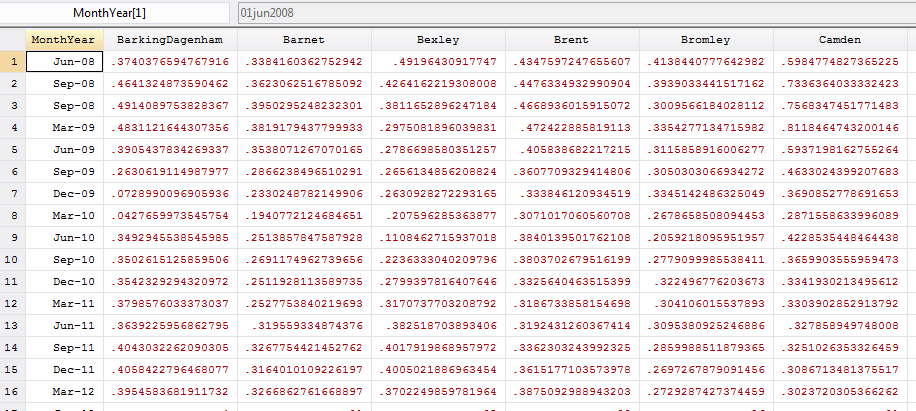
\includegraphics[width=5in]{data.PNG}
\end{frame}

\begin{frame}
  \frametitle{Transforming Data}
  \framesubtitle{}
Our data is too wide: we can use the -reshape- command to switch between ``wide" and ``long" formats. First we need to give the borough coloums a common prefix, then we can tell reshape to create a new variable. Attempting this also lets us know that we have two records for September 2008


\lstinputlisting[linerange={lstart-lend}]{../../stata/logs/foCrime_reshape.log}

\end{frame}






\begin{frame}
  \frametitle{Data types}
  \framesubtitle{}
The reason why Stata thinks our fear of crime variable is a string is that some of the values have \% characters (probably an artefact of inconsistent Excel cell formatting).

\smallskip

We can remove these using the -subinstr- command

\lstinputlisting[linerange={lstart-lend}]{../../stata/logs/destring.log}
\end{frame}

\begin{frame}
  \frametitle{}
  \framesubtitle{}
  \begin{itemize}
    \item 
  \end{itemize}
\end{frame}

\begin{frame}
  \frametitle{}
  \framesubtitle{}
  \begin{itemize}
    \item 
  \end{itemize}
\end{frame}

\begin{frame}
  \frametitle{References}
\bibliography{stata.bib}
\bibliographystyle{plain}
\end{frame}


\end{document}